\begin{columns}
  \begin{column}{0.5\textwidth}
    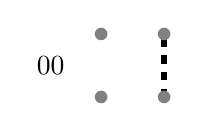
\begin{tikzpicture}[scale=0.8] % (0, 0) -> (0, 0) or (1, 1)
      \draw[line width=2, line cap=round, white]
       (-1,0)--(0,0)
       (-1,1)--(0,1)
      ;
      \node at (-0.8,0.5) {$\indxxx 00$};
      \draw[line width=2, dashed] (1,0)--(1,1);
      \fill[gray] (0,0) circle (0.1) (1,0) circle (0.1) (0,1) circle (0.1) (1,1) circle (0.1);
      \end{tikzpicture}
      \\~\\
      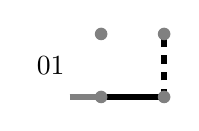
\begin{tikzpicture}[scale=0.8] % (0, 1) -> (0, 1) or (1, 2)
      \draw[line width=2, line cap=round, white]
       (-1,0)--(0,0)
       (-1,1)--(0,1)
      ;
      \node at (-0.8,0.5) {$\indxxx 01$};
      \draw[line width=2, gray!100] (-0.5,0)--(0,0);

      \draw[line width=2] (0,0)--(1,0);
      \draw[line width=2, dashed] (1,0)--(1,1);
      \fill[gray] (0,0) circle (0.1) (1,0) circle (0.1) (0,1) circle (0.1) (1,1) circle (0.1);
      \end{tikzpicture}
      \\~\\
      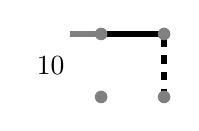
\begin{tikzpicture}[scale=0.8] % (1, 0) -> (1, 0) or (2, 1)
      \draw[line width=2, line cap=round, white]
       (-1,0)--(0,0)
       (-1,1)--(0,1)
      ;
      \node at (-0.8,0.5) {$\indxxx 10$};
      \draw[line width=2, gray!100] (-0.5,1)--(0,1);

      \draw[line width=2] (0,1)--(1,1);
      \draw[line width=2, dashed] (1,0)--(1,1);
      \fill[gray] (0,0) circle (0.1) (1,0) circle (0.1) (0,1) circle (0.1) (1,1) circle (0.1);
      \end{tikzpicture}
      \\~\\
      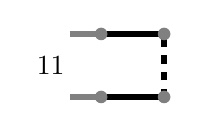
\begin{tikzpicture}[scale=0.8] % (1, 1) -> (1, 0) or (2, 1)
      \draw[line width=2, line cap=round, white]
       (-1,0)--(0,0)
       (-1,1)--(0,1)
      ;
      \node at (-0.8,0.5) {$\indxxx 11$};
      \draw[line width=2, gray!100]
       (-0.5,0)--(0,0)
       (-0.5,1)--(0,1)
      ;

      \draw[line width=2]
       (0,0)--(1,0)
       (0,1)--(1,1)
      ;
      \draw[line width=2, dashed] (1,0)--(1,1);
      \fill[gray] (0,0) circle (0.1) (1,0) circle (0.1) (0,1) circle (0.1) (1,1) circle (0.1);
      \end{tikzpicture}
  \end{column}
  \begin{column}{0.5\textwidth}  %%<--- here
    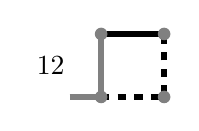
\begin{tikzpicture}[scale=0.8] % (1, 2) -> (1, 0), (1, 1), (2, 1), (2, 2)
      \draw[line width=2, line cap=round, white]
        (-1,0)--(0,0)
        (-1,1)--(0,1)
      ;
      \node at (-0.8,0.5) {$\indxxx 12$};
      \draw[line width=2, gray!100] (-0.5,0)--(0,0)--(0,1);

      \draw[line width=2] (0,1)--(1,1);
      \draw[line width=2, dashed] (0,0)--(1,0)--(1,1);
      \fill[gray] (0,0) circle (0.1) (1,0) circle (0.1) (0,1) circle (0.1) (1,1) circle (0.1);
    \end{tikzpicture}
    \\~\\
    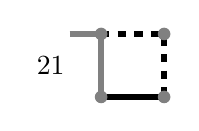
\begin{tikzpicture}[scale=0.8] % (2, 1) -> (0, 1), (1, 1), (1, 2), (2, 2)
      \draw[line width=2, line cap=round, white]
        (-1,0)--(0,0)
        (-1,1)--(0,1)
      ;
      \node at (-0.8,0.5) {$\indxxx 21$};
      \draw[line width=2, gray!100] (-0.5,1)--(0,1)--(0,0);

      \draw[line width=2] (0,0)--(1,0);
      \draw[line width=2, dashed] (0,1)--(1,1)--(1,0);
      \fill[gray] (0,0) circle (0.1) (1,0) circle (0.1) (0,1) circle (0.1) (1,1) circle (0.1);
    \end{tikzpicture}
    \\~\\
    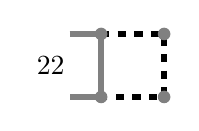
\begin{tikzpicture}[scale=0.8] % any + (1, 1)
      \draw[line width=2, line cap=round, white]
        (-1,0)--(0,0)
        (-1,1)--(0,1)
      ;
      \node at (-0.8,0.5) {$\indxxx 22$};
      \draw[line width=2, gray!100] (-0.5,1)--(0,1)--(0,0)--(-0.5,0);
      \draw[line width=2, dashed] (0,1)--(1,1)--(1,0)--(0,0);
      \fill[gray] (0,0) circle (0.1) (1,0) circle (0.1) (0,1) circle (0.1) (1,1) circle (0.1);
    \end{tikzpicture}
  \end{column}
\end{columns}